\documentclass[12pt, notitlepage]{article}
% \usepackage[bottom = 5cm, top = 5cm, left = 3cm, right = 3cm]{geometry}
\usepackage[margin = 1in]{geometry}
\usepackage[english]{babel}
\usepackage[utf8]{inputenc}
\usepackage[table]{xcolor}
\usepackage{graphicx, booktabs, tikz, csquotes, subcaption, enumitem, dcolumn, pdfpages, amsmath}
\usepackage[font=normalsize]{caption}%,labelfont=bf

\usepackage{endnotes}
\let\footnote=\endnote

\renewcommand*\rmdefault{ppl}

\usepackage{setspace}
\setstretch{1.5}

\usepackage[]{titlesec}
    \titleformat*{\section}{\large\bf}
    \titleformat*{\subsection}{\normalsize\it}

% Bibliography
% \usepackage[natbibapa]{apacite}
\usepackage[round]{natbib}
% \renewcommand{\bibliographytypesize}{\normalsize}
\setlength{\bibsep}{5pt}

\usepackage[colorlinks = TRUE, allcolors = blue]{hyperref}

\widowpenalty=10000
\clubpenalty=10000

\title{\Large Do TJ policies cause backlash?\\Evidence from street name changes in Spain}
\author{Francisco Villamil\footnote{Juan March Institute--Carlos III University of Madrid} \and Laia Balcells\footnote{Georgetown University}}
\date{\today}

%\usepackage[none]{hyphenat}

\usepackage{xr}
\externaldocument{appendix}

\begin{document}

\maketitle

\begin{abstract}
\setstretch{1.2}
Memories of old conflicts shape domestic politics long after these conflicts end. The debates about the Confederacy in the United States or the Francoist regime in Spain suggest that these are sensitive topics that might increase political polarization, particularly when transitional justice policies are implemented to address grievances. One such policy recently debated in Spain is the removal of public symbols linked to a past civil war and subsequent authoritarian regime (i.e., Francoism). However, the empirical evidence on their impact is still limited. This article attempts to fill this gap by exploring the impact of removing Francoist street names. Using cross-sectional and difference-in-differences analyses, we show that removing Francoist street names has increased electoral support to the new far-right party, Vox, mostly at the expense of the mainstream right-wing conservative party, PP. Results suggest that revisiting the past and trying to redress the victims' grievances can cause a backlash among those ideologically aligned with the perpetrator.

\vspace{10pt}
\noindent
% \textbf{Keywords:} transitional justice, voting, conflict memories, Spain

\end{abstract}
\setstretch{1.5}

\newpage
\section*{Introduction}

Memories of contested historical events shape domestic politics across the world.
In the United States, the Black Lives Matter movement has sparked a debate over Confederate symbols.% and the public display of a contentious past related to the Civil War and slavery.
The removal of these symbols, a transitional justice (thereafter, TJ) policy, is defended on the grounds that they represent ideas that are no longer acceptable, and that they constitute a roadblock to reconciliation.

Yet, the policy of symbol removal is not free of controversy.
In the South of the United States, there have been several instances of right-wing or white supremacist protests when statues of Confederates have been torn down.
%In some cases, these protests have turned violent.
The 2017 `Unite the Right' rally in Charlottesville, Virginia, opposing the removal of a Robert E Lee statue, escalated into violence and resulted in the death of one person when a white supremacist drove his car into a crowd of counter-protesters.

%In Germany, the co-leader of Alternative for Germany (AfD) dubbed the Berlin Holocaust Museum a ``monument of shame'' \citep{Laub:2018aa}. In Poland, the right-wing Law and Justice (PiS) party has recently changed the National Memory Law, ``threatening to prosecute anyone claiming that the Polish Nation was responsible for Nazi crimes'' \citep[][183]{Zubrzycki:2020aa}.

Do TJ symbolic policies cause a backlash in the form of a shift to radical (i.e. far right) positions?
This question is the focus of this article.
In particular, we explore a potential backlash effect of the removal of public symbols linked to the Francoist regime in Spain, where memories of the Civil War (1936--1939) still motivate fierce political debates. We exploit some of the changes brought about in Spain by the 2007 Law of Historical Memory, which introduced a mandate to remove Francoist symbols from public spaces, including street names. We study whether the renaming of streets generated an increase in electoral support for Vox, a relatively new far-right party.
%Originated from a split within the mainstream right-wing party (Partido Popular), Vox represents a hard version of Spanish nationalism.
%Its discourse glorifies Spain's imperial past and its national unity.
%It also condemns peripheral nationalisms and any attempt at redressing the official memory imposed by the Franco regime.
%In this study, we probe whether the removal of Francoist street names accounts for variation in support for Vox.

Our results support the authoritarian backlash hypothesis.
Cross-sectional analyses show there is a correlation between the removal of Francoist street names and electoral support for Vox in Spanish 2019 elections.
Also, in order to get closer to a causal identification, we implement a difference-in-difference (DiD) design where we explore the impact of Francoist street name removals on the growth of Vox electoral support between June 2016 and April 2019 elections.
Focusing only on a subset of municipalities that still had Francoist street names in June 2016, we show that Vox support increased around 6\% more in municipalities where there was a removal of Francoist street names between June 2016 and April 2019 than in places without name removals.
Interestingly, we find that support for the Partido Popular (PP) decreased 8\% more in those same municipalities, while support for the the socialist party (PSOE) did not vary, suggesting a potential link to increased asymmetric polarization.

%The politics of memory and the revision of a country's history are key issues in contemporary politics.
%National traditions and symbols across the world are being criticized because of their racial or ideological overtones.
%Even though those who support these revision policies usually claim that they promote reconciliation, our argument is that can also have the unintended side effect of increasing political polarization.

\section*{The consequences of TJ policies}

After regime transitions or violent episodes, states often confront the need to come to terms with the past.
To this end, states rely on different TJ policies, including legal responses such as trials and amnesties or setting up truth commission, museums, or memorials \citep{De-Brito:2001aa, Elster:2004aa, Balasco:2013aa}. All these measures aim to serve justice, redress grievances, and avoid the relapse of conflicts. However, the short-term and long-term and consequences of TJ are not clear.

Many scholars praise TJ policies in postconflict contexts, arguing that these policies increase the prospect for democracy \citep{Elster:2004aa, Sikkink:2007aa} and reduce the risk of future conflict by increasing accountability for past violence and repression \citep{Kim:2010aa, Meernik:2010aa}. TJ policies attempt to redress individual grievances and collective grudges \citep{Scharf:1997aa, Akhavan:1998aa, Hayner:2001aa}.

Other authors argue that the positive view on TJ policies is overly optimistic, and that there is scant evidence in support of a beneficial effect of TJ \citep{Mendeloff:2004aa, Thoms:2010aa, Daly:2011aa}.
Some works even claim that TJ policies can have a negative effect on reconciliation and conflict, because the exclusive reliance on prosecution and accountability can bring about social tensions in divided societies \citep{Goldsmith:2003aa, Snyder:2004aa}.
%\footnote{The idea that TJ policies might intensify old hatreds and divisions was precisely one of the arguments held by conservative sectors in Spain against the 2007 Law of Historical Memory.}
%Indeed, the debates about the past related to these TJ policies seem to have played a meaningful role in building a successful electoral discourse among populist right-wing parties in some European countries \citep{Martin:2020aa}.

%Previous research has paid close attention to the formal justice mechanisms of TJ policies, but we know much less about more informal measures of TJ and their effects on public opinion or voting behavior.
%Two recent works constitute a partial exception to this gap.
Some recent works have tried to shed light on this debate. \cite{Capoccia:2020aa} study the effects of TJ trials on prodemocratic attitudes in West Germany, and find heterogenous effects depending on the type of punishment and the ethnic identity of the defendants.
\cite{Balcells:2020aa}, for their part, study the impact of TJ museums in a field experiment. They find that visiting a TJ museum in Chile can have a reconciliatory effect, suggesting a positive aspect of the politics of memory.
We contribute to this literature by exploring the effects of a particular subset of TJ policies, the removal of symbols from public spaces, on voting behavior in Spain. In particular, we focus on the removal of Francoist street names. Street renaming, just like the removal of statues and other symbols or the building of museums and establishment of historical markers,\citep{Ward2021} are a form of what \citet{Aguilar:2011aa} call ``symbolic Transitional Justice''. Symbolic TJ is very much intertwined with the politics of memory, which involve ``the shaping of collective memory by political actors and institutions'' \citep[][176]{Zubrzycki:2020aa}, are a crucial component of these policies. While there has been significant research on other aspects of TJ policies such as trials, reparations, or lustration, the study of symbolic TJ is still quite underdeveloped. We are interested in testing the backlash hypothesis, namely, that removing public symbols will mobilize and radicalize those who are ideologically closer to these symbols.

If this hypothesis is true in the context of Spain, we expect to find a local increase in far-right voting in those areas where these TJ symbolic policies were applied.

\section*{Conflict memories and authoritarian backlash in Spain}

%We exploit two recent phenomena in Spanish politics: the consequences of the Law of Historical Memory and the recent rise of a far-right party, Vox.%, whose discourse rests heavily on the version of Spanish nationalism supported by Francoism.

In Spain the Law of Historical Memory, promoted by a left-wing (PSOE) government and passed by the Congress of Deputies in 2007, was an attempt to redress long-held grievances by the victims of the Civil War and the Francoist regime.
Among other things, it included provisions for the removal of Francoist symbols from public spaces, such as street names and monuments.

Some local governments had already changed Francoist street names right after the transition to democracy.
%For instance, the \textit{Paseo de la Castellana} and the \textit{Avinguda Diagonal}, two of the main arteries of Madrid and Barcelona, respectively, were named \textit{Avenida del Generalísimo Franco} until 1979.
However, these changes depended on an active decision made at the local level.
In many places, either because the civil war/Francoist issue was less salient or because local politicians actively rejected the change, many streets were still named after Francoist symbols or leaders.
The 2007 Law prompted local governments to act and offered local associations a legal platform to pressure their local councils.% to promote street name changes.
%\footenote{In fact, the Law of Historical Memory promoted and funded local `memory associations' that reviewed the local history and organized the exhumation of local mass graves.}

These policies were hotly contested by particular sectors of Spanish society. Even from the very first years of democratic rule, rightist parties rejected the change of street names or the removal of public monuments by saying that revisiting history only brought old-seated divisions back \citep[e.g.][]{Fuente:1980aa}.
\footnote{The exhumation of Francisco Franco from the Valley of the Fallen in late 2019 is probably the latest high-key example of the implementation of this law and the political tension it brought about \citep{Taladrid:2019aa}.}
By the late 2000s, even if the 2007 Law had a broad support in Spanish society, a significant proportion of the population still disagreed with its provisions \citep{Aguilar:2011aa}.

To analyze the effect of TJ policies aimed at removing symbols, we focus on electoral support for Vox as our measure for far-right ideological preferences.
Vox is a relatively new party in Spain which promotes a discourse based on authoritarian conservatism and a hard-line version of Spanish nationalism. It shares with other populist right-wing parties in Europe a nativist ideology and a rejection of immigration, gender policies, and the social welfare state \citep{Turnbull-Dugarte:2019aa, Turnbull-Dugarte:2020aa}.
%The most relevant aspect of its discourse for this study is the use they made of the issue of historical memory in Spain.
Characterizing the Law of Historical Memory as an instrument of leftist propaganda, Vox campaigned on the national unity of Spain as a way of leaving behind historical divisions and enacted the figure of Francisco Franco as an important political leader who brought peace and stability to the country. This discourse mirrors the `forgetting` policy developed by Franco in the postwar period \citep{Palomares:2004aa}.

We make use of these two events to assess whether the politics of memory in Spain caused a backlash towards positions closer to the ideology of the Francoist regime. In particular, we measure whether the renaming of streets led to increased  support for Vox.
%Our expectation is that the relationship will be positive, supporting the backlash hypothesis.

\section*{Empirics}

We first test whether the removal of Francoist streets since 2001 is correlated with higher support for Vox in both 2019 elections.
We also implement a DiD analysis on the increase in electoral support for Vox between June 2016 and April 2019 elections, using the removal of Francoist street names as our main independent variable and limiting the sample only to those municipalities that still had Francoist street names in June 2016.

\subsection*{Francoist street name removal}

To build our main independent variable, we downloaded data identifying all the streets in Spain at different points in time from the National Statistical Institute \citep{INE:2020aa}.
In particular, the INE offers data for every six-month period since December 2010,\footnote{Specifically, it offers the official data for June 30th and December 31st.} plus a snapshot of the streets and their names existing in July 2001.
We track the change in street names over time using the official ID number for each street.

Using this setup, we identified streets named after Francoist symbols or figures.
We used the list published by the Madrid City Council in 2017, following a report by a specially designated commission\footnote{The full list is available online at https://bit.ly/37cLGgk (accessed 26/11/2020).}, and expanded it selecting from street names that were often changed during this period.
% Indeed, among all the changes between 2001 and 2020, the five most commonly removed street names were all key Francoist figures: `Jose Antonio', `Calvo Sotelo', `General Mola', `Generalísimo', and `General Franco'.
We include in the Appendix the full list of Francoist street names.
We use a binary indicator of Francoist street name removal, except for the initial cross-sectional models where we also show results using a continuous measure.\footnote{See section~\ref{app:treatment_strength} in the appendix for more details.}
% In the appendix, we show that the results do not change if we use a continuous measure (logged number of changes) instead.

Figure~\ref{fig:changes_time} shows the number of changes during every six-month period, while figure~\ref{fig:fs_year} shows yearly data on the share of all the streets with Francoist names.
There was an increase in Francoist name removal after 2016, precisely the period we use in our DiD analyses.
Two main factors probably explain these trends.
First, the initiative to change street names was local and any legal battle or pressure campaign would take time.
For example, in mid-2016, Olmedo, Valladolid, was the first municipality to be condemned for not complying with the 2007 Law of Historical Memory \citep{El-Norte-de-Castilla:2016aa}.
Around the same time, many municipalities began facing trials after being sued by local associations.
%, such as Llanes, Asturias \citep{El-Comercio:2016aa}.
Second, the decrease in votes for the mainstream right-wing party in the 2015 local and regional elections changed the balance of power which, together with a general increase in the salience of this issue, meant more institutional activity in this direction \citep[e.g.][]{Vazquez:2016aa, El-Comercio:2016ab}.

\begin{figure*}[htb!]
\centering

  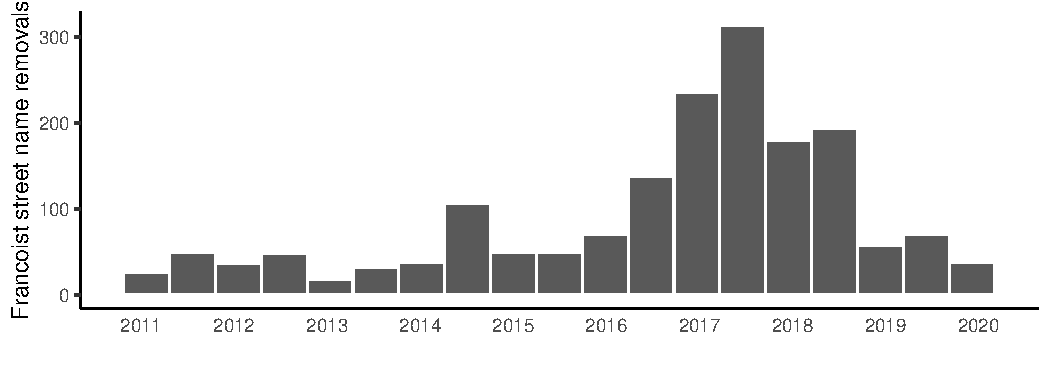
\includegraphics[width = 0.8\textwidth]{img/changes_by_year}

  \caption{Number of Francoist street name removals over time}\label{fig:changes_time}

\end{figure*}

\begin{figure*}[htb!]
\centering

  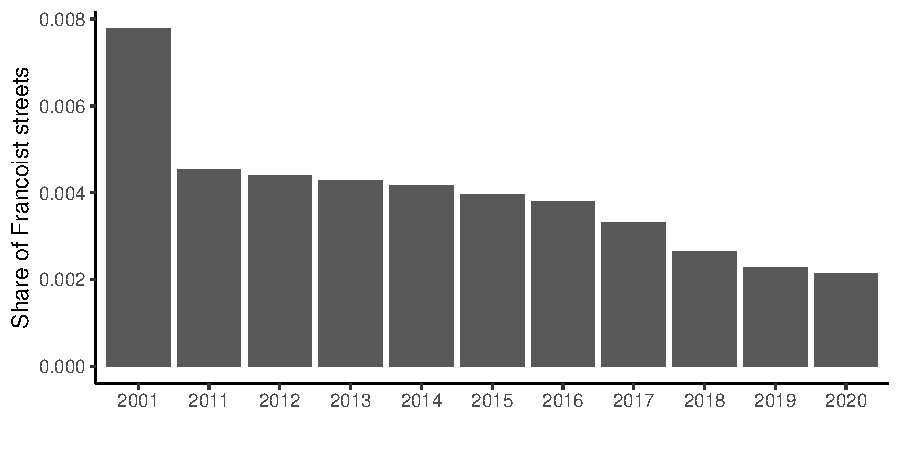
\includegraphics[width = 0.7\textwidth]{img/fs_by_year}

  \caption{Share of streets with Francoist street names over time}\label{fig:fs_year}

\end{figure*}

However, the post-2016 increase could bias the results if it was related to political dynamics that also explain the change in political preferences.
We discuss this issue in more depth in the results section, but the data suggests this is not the case.
We discuss at length the differences between municipalities in and out of the sample in the appendix (section~\ref{app:treated_vs_control_vs_outsample}).% we show that most of the municipalities that removed Francoist street names were small municipalities that had more Francoist street names to start with, and mostly in provinces in the central regions of Spain, which is in line with the factors discussed above.

\subsection*{Vox electoral support}

We exploit support for Vox as our main dependent variable.%, using it as a proxy for an authoritarian backlash in political preferences.
We obtained the data from the Spanish Ministry of Interior,\footnote{Results are available at \href{http://www.infoelectoral.mir.es/}{http://www.infoelectoral.mir.es/} (accessed 03/12/2020).}
and calculated the share of valid votes for Vox in each municipality.

In the DiD analyses, we also use as dependent variables the electoral share for the two mainstream parties, the right-wing Popular Party (\textit{Partido Popular}, PP) and the Spanish Socialist Workers' Party (\textit{Partido Socialista Obrero Español}, PSOE), in order to capture the local shift in political preferences.
%Specifically, given that we are interested in a potential authoritarian backlash among conservative individuals, we want to explore whether the removal of Francoist street names is related to a general shift to the right or an increase in political polarization.

\subsection*{Control variables}

We include a series of control variables that can be related to electoral support for Vox.
In the cross-sectional analyses on electoral results in 2019, we include turnout, the (logged) population in the 2011 census, and the local unemployment rate in January 2011.
In the DiD analyses, we include population, unemployment rate in January 2016, the (logged) number of Francoist streets in June 2016, and a dummy indicating whether a leftist mayor was elected in the 2015 local elections.
In every case, we also include fixed effects at the region level (Autonomous Communities).

\subsection*{Models}

%We build two sets of models.
The cross-sectional analyses use OLS regression on the vote share of Vox in both 2019 elections (April and November), using as the main independent variable binary and continuous indicators of street name removal between June 2001 and December 2018, the larger period for which we have data.
We only include in the sample municipalities that had at least one street with Francoist name in June 2001.
The models are defined as:

\begin{equation}
  Vox_Share{i} = \beta_0 + \beta_1 Removal_{i} + \beta^\top \mathbf{x}_{i} + \alpha_{i} + \epsilon_{i}
\end{equation}

In the DiD analyses, we also run OLS using the electoral support for Vox, PP, and PSOE in June 2016 and April 2019 elections as the dependent variable, and an indicator of street name removal between June 2016 and December 2018 as our main independent variable.
The model is defined as:

\begin{equation}
\begin{split}
  Share_{it} =& \beta_0 +\\
  &\beta_1 Removal_{it} + \beta_2 April2019_{it} + \beta_3 (Removal_{it} \times April2019_{it}) +\\
  &\beta^\top \mathbf{x}_{it} + \alpha_{it} + \epsilon_{it}
\end{split}
\end{equation}

Where the effect of street name removals is captured by $\beta_3$, or the interaction between the time and removal dummies.
In these models, we only compare municipalities that had at least one street with Francoist name in June 2016. Table~\ref{tab:sample_trt} summarizes this classification.\footnote{In order to use the same sample of municipalities in all models, we limit the sample to those municipalities where Vox participated in 2016 elections. Results do not change if we use the full available sample for each party.}

\begin{table}[!htbp] \centering
\caption{DiD sample classification}
\label{tab:sample_trt}
\small
\begin{tabular}{lcc}
\\[-1.8ex]\hline
\hline \\[-1.8ex]
\multicolumn{1}{p{3cm}}{\hspace{3cm} Francoist names} & \multicolumn{2}{p{3.5cm}}{Removed Francoist names, 2016--2018?}\\
in June 2016? & No & Yes \\
\cline{2-3} \\[-1.8ex]
No & 6455 & 0 \\
 & (100\%) & (0\%) \\
Yes (DiD sample) \hspace{2cm} & 1184 & 454 \\
 & (72\%) & (28\%) \\
\\[-1.8ex]\hline
\hline \\[-1.8ex]
\multicolumn{3}{c}{\parbox[t]{0.55\textwidth}{\textit{Note:} Row percentages. Changes in 2016--2018 refer to the period between 01/07/2016 and 31/12/2018.}}\\
\end{tabular}
\end{table}


Limiting the sample implies that the the control group---those municipalities that did not change street names during this period---is probably more rightist than the average (compared to municipalities out of the sample), as more leftist municipalities are more likely to have already changed Francoist street names before mid-2016.
Indeed, some municipalities that still had not changed Francoist names by late 2018 were portrayed as the `resistance' to the Law of Historical Memory \citep{Blanco-Elipe:2018aa}, as they actively avoided doing so.
This dodging of the Law was possible either because of delays in the legal procedures or some form of `foot-dragging' by local authorities.
Because of this, we think that, if anything, the selection bias should go against the backlash hypothesis, in the sense that the control group is comprised by municipalities where Vox is likely to have grown more between 2016 and 2019.
We provide further empirical evidence on this in the appendix (section~\ref{app:treated_vs_control_vs_outsample}) as well as a test of the parallel trends assumption (section~\ref{app:robustness_did}).
% We also include a series of additional models in the appendix to test the robustness of the results.

%We also include a series of additional models in the appendix to test the robustness of the results.
%In particular, we include pre-treatment placebos to test the parallel trends assumption, include two different specifications of the name removal variable (in continuous form, and extending changes to the first half of 2019), and restrict the sample to municipalities where Vox got more than 0 votes in June 2016.

\section*{Results}

Table~\ref{tab:cs} shows the results of the cross-sectional analyses.
The first two columns show that the removal of Francoist street names during the last two decades, between June 2001 and December 2018, is correlated with a higher electoral support for Vox in both April and November 2019 elections.
Columns 3 and 4 repeat these analyses with a limited sample of municipalities that still had Francoist street names in June 2001, and also show a positive correlation between street name changes and Vox electoral support.


% Table created by stargazer v.5.2.2 by Marek Hlavac, Harvard University. E-mail: hlavac at fas.harvard.edu
% Date and time: Tue, Jun 15, 2021 - 19:16:21
% Requires LaTeX packages: dcolumn 
\begin{table}[!htbp] \centering 
  \caption{Francoist street name removal and electoral support for Vox} 
  \label{tab:cs} 
\small 
\begin{tabular}{@{\extracolsep{-20pt}}lD{.}{.}{-3} D{.}{.}{-3} D{.}{.}{-3} D{.}{.}{-3} } 
\\[-1.8ex]\hline 
\hline \\[-1.8ex] 
\\[-1.8ex] & \multicolumn{1}{c}{\footnotesize Apr 2019} & \multicolumn{1}{c}{\footnotesize Nov 2019} & \multicolumn{1}{c}{\footnotesize Apr 2019} & \multicolumn{1}{c}{\footnotesize Nov 2019} \\ 
\\[-1.8ex] & \multicolumn{1}{c}{(1)} & \multicolumn{1}{c}{(2)} & \multicolumn{1}{c}{(3)} & \multicolumn{1}{c}{(4)}\\ 
\hline \\[-1.8ex] 
 (Intercept) & 0.120^{***} & 0.213^{***} & 0.119^{***} & 0.211^{***} \\ 
  & (0.018) & (0.020) & (0.018) & (0.020) \\ 
  Francoist street name removal (log. no) & 0.003^{+} & 0.005^{**} &  &  \\ 
  & (0.002) & (0.002) &  &  \\ 
  Francoist street name removal (dummy) &  &  & 0.005^{*} & 0.008^{**} \\ 
  &  &  & (0.002) & (0.003) \\ 
  Unemployment 2019 & 0.042 & 0.139^{*} & 0.043 & 0.141^{*} \\ 
  & (0.047) & (0.058) & (0.047) & (0.058) \\ 
  Turnout April 2019 & -0.020 &  & -0.020 &  \\ 
  & (0.020) &  & (0.020) &  \\ 
  Turnout Nov 2019 &  & -0.086^{***} &  & -0.086^{***} \\ 
  &  & (0.023) &  & (0.023) \\ 
  Log. Population & 0.001^{+} & 0.003^{***} & 0.002^{*} & 0.003^{***} \\ 
  & (0.001) & (0.001) & (0.001) & (0.001) \\ 
 \hline \\[-1.8ex] 
CCAA Fixed Effects & \multicolumn{1}{c}{Yes} & \multicolumn{1}{c}{Yes} & \multicolumn{1}{c}{Yes} & \multicolumn{1}{c}{Yes} \\ 
Observations & \multicolumn{1}{c}{2,164} & \multicolumn{1}{c}{2,165} & \multicolumn{1}{c}{2,164} & \multicolumn{1}{c}{2,165} \\ 
R$^{2}$ & \multicolumn{1}{c}{0.291} & \multicolumn{1}{c}{0.317} & \multicolumn{1}{c}{0.292} & \multicolumn{1}{c}{0.318} \\ 
Adjusted R$^{2}$ & \multicolumn{1}{c}{0.283} & \multicolumn{1}{c}{0.310} & \multicolumn{1}{c}{0.284} & \multicolumn{1}{c}{0.311} \\ 
\hline 
\hline \\[-1.8ex] 
\multicolumn{5}{c}{\parbox[t]{0.8\textwidth}{\textit{Note:} $+ p<0.1; * p<0.05; ** p<0.01; *** p<0.001$. The main independent variable refers to the removal of Francoist street names between June 2001 and December 2018. Models 3 and 4 only include municipalities that had Francoist street names in June 2001.}} \\ 
\end{tabular} 
\end{table} 


In the appendix (see section~\ref{app:additional_cs}), we show that the results do not change significantly when looking only at street name removals after the 2007 Law of Historical Memory was passed, namely, between 2011 and 2018.
We also show that there is no correlation between these name changes and the change in support for Vox between April and November 2019 elections, which suggests that any local effect due to a backlash over the politics of memory took place prior to April 2019.
Finally, we also include additional models looking at street name removals over different periods.

To get closer to identifying the causal effect of street name changes, we develop a DiD setup where we analyze the increase in electoral support for Vox between 2016 and 2019 elections, together with the main two parties, PSOE and PP.
Table~\ref{tab:main_did} shows the results of these analyses.
% Each of the three columns shows the results for the same model using electoral support for the three different parties.
In order to see the results more clearly, figure~\ref{fig:main_did} shows the simulated DiD estimate of the Francoist street name removal, using the models with control variables.
%In other words, the effect of the street name removal on the change in electoral support for these parties between 2016 and 2019.


% Table created by stargazer v.5.2.2 by Marek Hlavac, Harvard University. E-mail: hlavac at fas.harvard.edu
% Date and time: Thu, May 27, 2021 - 17:29:25
% Requires LaTeX packages: dcolumn 
\begin{table}[!htbp] \centering 
  \caption{Francoist street name removal and increase in electoral support for parties} 
  \label{tab:main_did} 
\small 
\begin{tabular}{@{\extracolsep{-20pt}}lD{.}{.}{-3} D{.}{.}{-3} D{.}{.}{-3} } 
\\[-1.8ex]\hline 
\hline \\[-1.8ex] 
\\[-1.8ex] & \multicolumn{1}{c}{VOX} & \multicolumn{1}{c}{PP} & \multicolumn{1}{c}{PSOE} \\ 
\\[-1.8ex] & \multicolumn{1}{c}{(1)} & \multicolumn{1}{c}{(2)} & \multicolumn{1}{c}{(3)}\\ 
\hline \\[-1.8ex] 
 (Intercept) & -1.470^{**} & 56.375^{***} & 34.870^{***} \\ 
  & (0.451) & (0.922) & (0.876) \\ 
  Francoist street name removal & -0.132 & 1.158^{*} & -0.159 \\ 
  & (0.262) & (0.476) & (0.453) \\ 
  Election April 2019 & 12.319^{***} & -17.406^{***} & 4.629^{***} \\ 
  & (0.167) & (0.338) & (0.320) \\ 
  Francoist removal $\times$ April 2019 & 0.724^{*} & -1.405^{*} & -0.434 \\ 
  & (0.352) & (0.639) & (0.607) \\ 
 \hline \\[-1.8ex] 
Controls & \multicolumn{1}{c}{Yes} & \multicolumn{1}{c}{Yes} & \multicolumn{1}{c}{Yes} \\ 
CCAA Fixed Effects & \multicolumn{1}{c}{Yes} & \multicolumn{1}{c}{Yes} & \multicolumn{1}{c}{Yes} \\ 
Observations & \multicolumn{1}{c}{2,310} & \multicolumn{1}{c}{3,223} & \multicolumn{1}{c}{3,242} \\ 
R$^{2}$ & \multicolumn{1}{c}{0.768} & \multicolumn{1}{c}{0.720} & \multicolumn{1}{c}{0.482} \\ 
Adjusted R$^{2}$ & \multicolumn{1}{c}{0.766} & \multicolumn{1}{c}{0.717} & \multicolumn{1}{c}{0.478} \\ 
\hline 
\hline \\[-1.8ex] 
\multicolumn{4}{c}{\parbox[t]{0.75\textwidth}{\textit{Note:} $+ p<0.1; * p<0.05; ** p<0.01; *** p<0.001$. Only municipalities that had at least one street with a Francoist name in $t_{0}$ were included in the sample.}} \\ 
\end{tabular} 
\end{table} 


\begin{figure*}[htb!]
\centering

  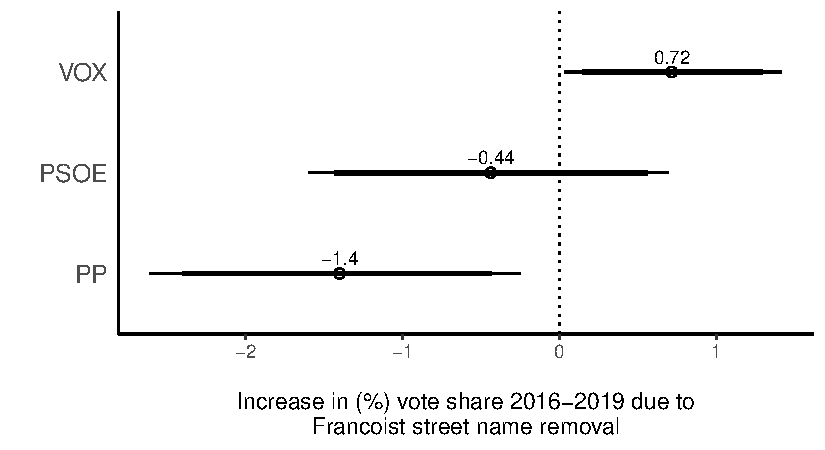
\includegraphics[width = 0.6\textwidth]{img/DiD_estimates}

  \caption{DiD estimates of Francoist street name removal on vote change, obtained from 1000 simulations. Points show the mean estimate, bars indicate 90\% and 95\% CIs.}\label{fig:main_did}

\end{figure*}

Results support the idea that the changes caused a backlash.
On the one hand, in municipalities where Francoist street names were removed, Vox increased its support 0.7 points more.
Considering that the nation-wide electoral share of Vox in April 2019 was 10.3\%, this effect is significant: the change in electoral support was around 6\% higher in these municipalities.
On the other hand, the removal of Francoist street names is related to an even higher decrease in electoral support for PP, of almost 1.5 points.
However, it did not have any significant effect on electoral support for PSOE, which suggests the change in political preferences took place among rightist individuals.

These results could be confounded if the removal of Francoist street names was explained by the same factors that also explain a shift to far-right preferences.
One possibility is that these street name changes, which took place relatively late, took place in more conservative areas where Spanish nationalism was stronger.
We believe that any selection bias in the sample should be in the opposite direction from the results.
Moreover, if the concern above were true, we should see different trends before 2016 between municipalities that later had a change and those that did not.
Figure~\ref{fig:par_trends_norm} shows normalized electoral trends among control and treated groups for PP and Vox, and we include in the appendix much more detailed models analyzing the parallel trends assumption for Vox, PP, and PSOE.

We also show in the appendix results including the main independent variable in continuous form (logged number of street name removals), restricting the sample to municipalities where Vox had more than 0 votes in 2016, and changing the independent variable so it also registers changes that were registered in the first half of 2019, to account for possible delays in the official data.
Results do not change in any of these specifications (see section~\ref{app:robustness_did}), and results from first-difference models go in the same direction (section~\ref{app:first_diff}).


\begin{figure*}[htb!]
\centering

  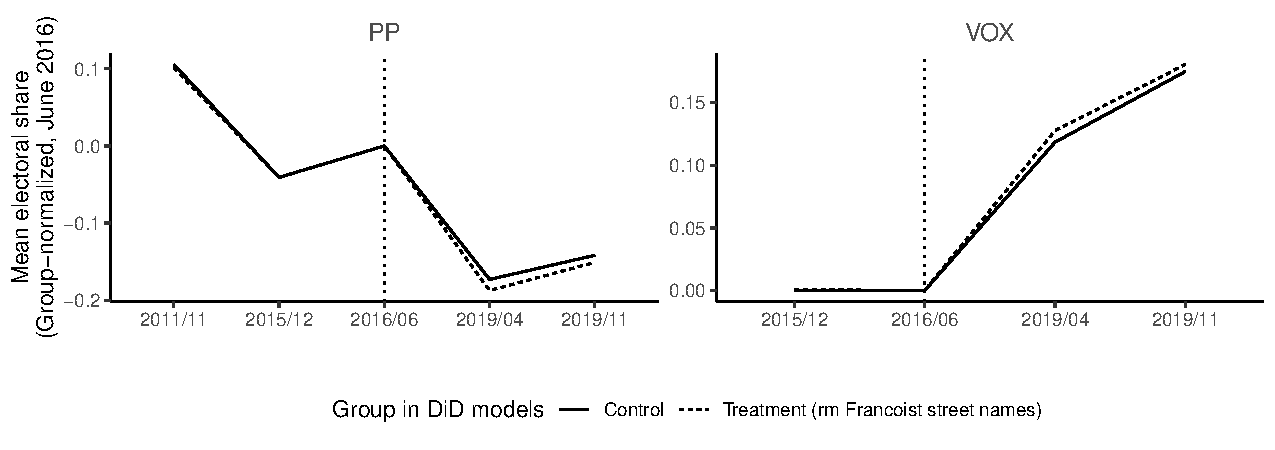
\includegraphics[width = \textwidth]{img/par_trends_norm}

  \caption{Pre- and post-treatment trends in Vox and PP electoral share}\label{fig:par_trends_norm}

\end{figure*}

\section*{Conclusion}

In this article, we have explored the political effect of the removal of Francoist street names in Spain.
Our results suggest that this policy can cause a backlash. In particular, using local-level data, we find a short-term positive effect of these changes on the increase in support for the far-right party Vox, a party that has recently gained steam with a discourse grounded in an authoritarian and exclusive version of Spanish nationalism.

The results from our analyses echo recent debates about symbolic TJ policies and memories of past conflicts in other countries. For example, the debate in the United States over the Confederate symbols shows that this type of policies can generate political instability and even violence. And, in Ukraine, the removal of Soviet monuments has lead to increased support for pro-soviet political parties \citep{Rozenas:2021}. While we do not take a normative stand agains these policies, we show that there is room for concern: revisiting the past and trying to redress the victims' grievances might cause a backlash among those ideologically closer to the perpetrator, leading to increased (asymmetric) political polarization. This backlash can perhaps be remedied by actions of other political parties -- for example, countering the narrative of the opponents or compensating them in other ways, but the extent to which such remedial policies would work is out of the scope of this paper.

%Far from arguing against these types of policies, we think it is important to be aware of these potentially undesired effects when designing transitional justice policies. Specifically, two aspects merit further attention:
Also, here we show evidence of a short-term backlash effect. Yet, we do not know what happens in the longer term, particularly whether these policies produce a reconciliation effect down the road. Finally, even if the removal of public symbols might cause backlash, this might not be the case for other TJ policies. For instance, recent research shows that TJ museums might have a positive effect on reconciliation \citep{Balcells:2020aa} and that the overall effect of TJ depends on the balance between different measures \citep{Olsen:2010aa, Loyle:2017aa}

All in all, this article focuses on a relatively unexplored question. Exploiting recent political events in Spain, we offer empirical evidence suggesting that, in the short run, symbolic transitional justice policies might have an unintended effect: an increased support for political actors siding with the former regime or perpetrators of violence. In Spain, this is the case of the far-right.

\newpage
\begingroup
\parindent 0pt
\parskip 2ex
\def\enotesize{\normalsize}
\theendnotes
\endgroup

\clearpage
\bibliographystyle{rap}
\bibliography{REF}

\newpage
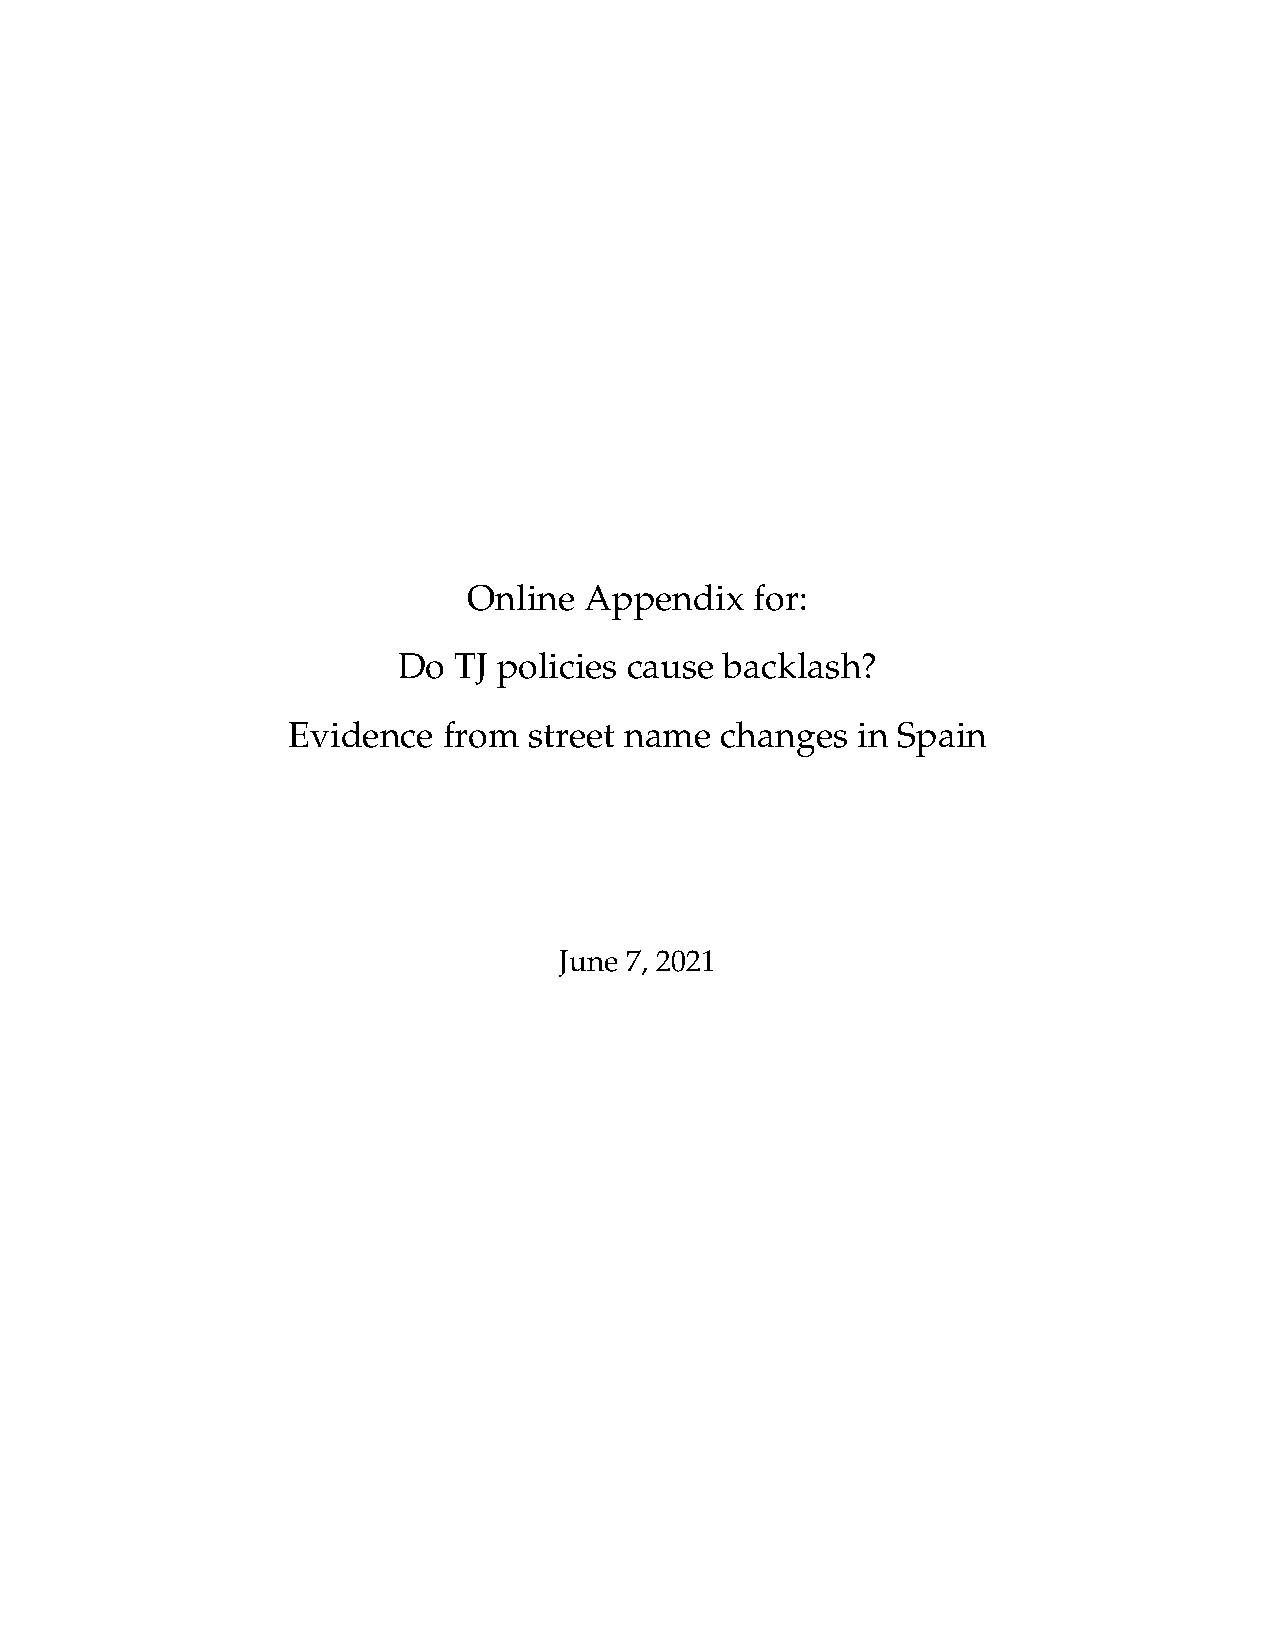
\includepdf[pages=-]{appendix.pdf}

\end{document}
